\subsection{Access control flows}\label{sec:access-control-flows}
The access control flow of the proposed system can be broken down into three stages:
\begin{enumerate*}[label=(\roman*)]
    \item \textit{Authentication},
    \item \textit{Access Policy Evaluation} and
    \item \textit{Access Policy Enforcement}.
\end{enumerate*}

All of these three stages can be identified in both use cases UC-1 and UC-2. UC-17 and UC-18 also have steps for policy evaluation and policy enforcement during their processing. However, the flow in each stage is adapted to the given use case.

\subsubsection{Authentication}
In this stage, the user identifies and authenticates themselves to the \acrshort{aaserver}. This is the first stage of the access control flow and is only preceded by the user clicking a login button or approaching a door. The authentication is done via the FIDO2 protocol, but the flows during this stage are different during online login and when opening a door.

\paragraph{Authenticating online} During online authentication the Requester is a client application (internal or external). Even when the first step is made in the native application, the user must use a user agent to carry out the authentication on the \acrshort{aaserver}. When the user clicks a login button, the client application sends an \textit{Access request} message to the server, which contains these parameters: the \textit{client\_id}, the callback URL, the requested scopes (and if the client is a native application, also the \acrshort{pkce} code challenge). The \textit{client\_id} is immediately verified by the \acrshort{aaserver} and the other variables are temporarily saved for later use. User is then redirected to a login page, supplied by the \acrshort{aaserver}. 

User enters their \acrshort{uid} into the supplied form and chooses the authentication method they wish to use (either \textit{physical key} or \textit{smartphone}). The form data is sent back to the \acrshort{aaserver}, which requests a challenge from the User Directory. If the user selected physical key as their authentication method, the User directory generates a challenge, which is passed onto the user agent, signed by the authenticator and returned back via the \acrshort{aaserver} to the the User directory.

If the user selected smartphone as their authentication method, then the challenge created by the User directory is forwarded to the Authentication Front End, instead of the user agent. The messages between the \acrshort{aaserver} and the user agent/authentication front end have the form of standard WebAuthn requests and responses, as defined by~\cite{Balfanz2019Web1}. 
Once the User Directory receives the signed challenge, it verifies whether the signature was made with the private key belonging to the public key stored for the given \acrshort{uid}. It then informs the \acrshort{aaserver} whether the verification was successful or not.

In the last step of the Authentication stage, the \acrshort{aaserver} issues a signed and encrypted \acrshort{jwt} to the user agent/Authentication Front End. The purpose of this is to avoid repeated authentication prompts to the user in a short time span (a couple of hours). Once the user authenticates using an authenticator on certain user agent, they are not prompted to authenticate on the same user agent again, until the validity of the \acrshort{jwt} has expired.
 
Cookies could also be used for token-based authentication to the \acrshort{aaserver}. While there is not yet consensus on which technology should be used~\cite{Beltran2016CharacterizationProtocols, RajuRaghuwanshi2017JWTCookies}, \acrlong{jwt}s offer better support on mobile devices and are not vulnerable to Cross-site request forgery attacks.\footnote{\url{http://web.archive.org/web/20190521213404/https://campus.barracuda.com/product/webapplicationfirewall/doc/42049419/cookie-replay-attack/}, accessed 21 May 2019}

If the \acrshort{aaserver} receives a valid \acrshort{jwt} in the Access request, it does not carry out further authentication steps and proceeds directly to the Access Policy Evaluation stage. If the received \acrshort{jwt} is expired or otherwise invalid, the regular process described above applies.

Figure~\ref{fig:authentication-flow} illustrates this process in a sequence diagram. User authentication with a physical key is shown, when logging in online to an external application, which corresponds to UC-1. When authenticating with a smartphone and when using a \acrshort{pacs}, the flow would be slightly different.

\paragraph{Authenticating to a \acrshort{pacs}} 
When passing a physical checkpoint (described in UC-2), the authentication and policy evaluation must be speedy (as specified by RQ-20). The flow in this case must be adjusted, to fulfil this requirement.

The \acrshort{jwt} cannot be used and is omitted from the process. The authentication method selection form and the \acrshort{uid} input form are both omitted. Instead, the physical key is used as the default authentication method and the \acrshort{uid} is extracted directly from the authenticator. The signed challenge together with the \acrshort{uid} is forwarded to the User Directory, which looks up the \acrshort{uid}, verifies the challenge and informs the \acrshort{aaserver} about the outcome.

\newgeometry{left=1.2cm,right=1.2cm,top=1cm,bottom=1cm,footskip=.4cm}
\begin{sidewaysfigure}[tpb]
    \centering
    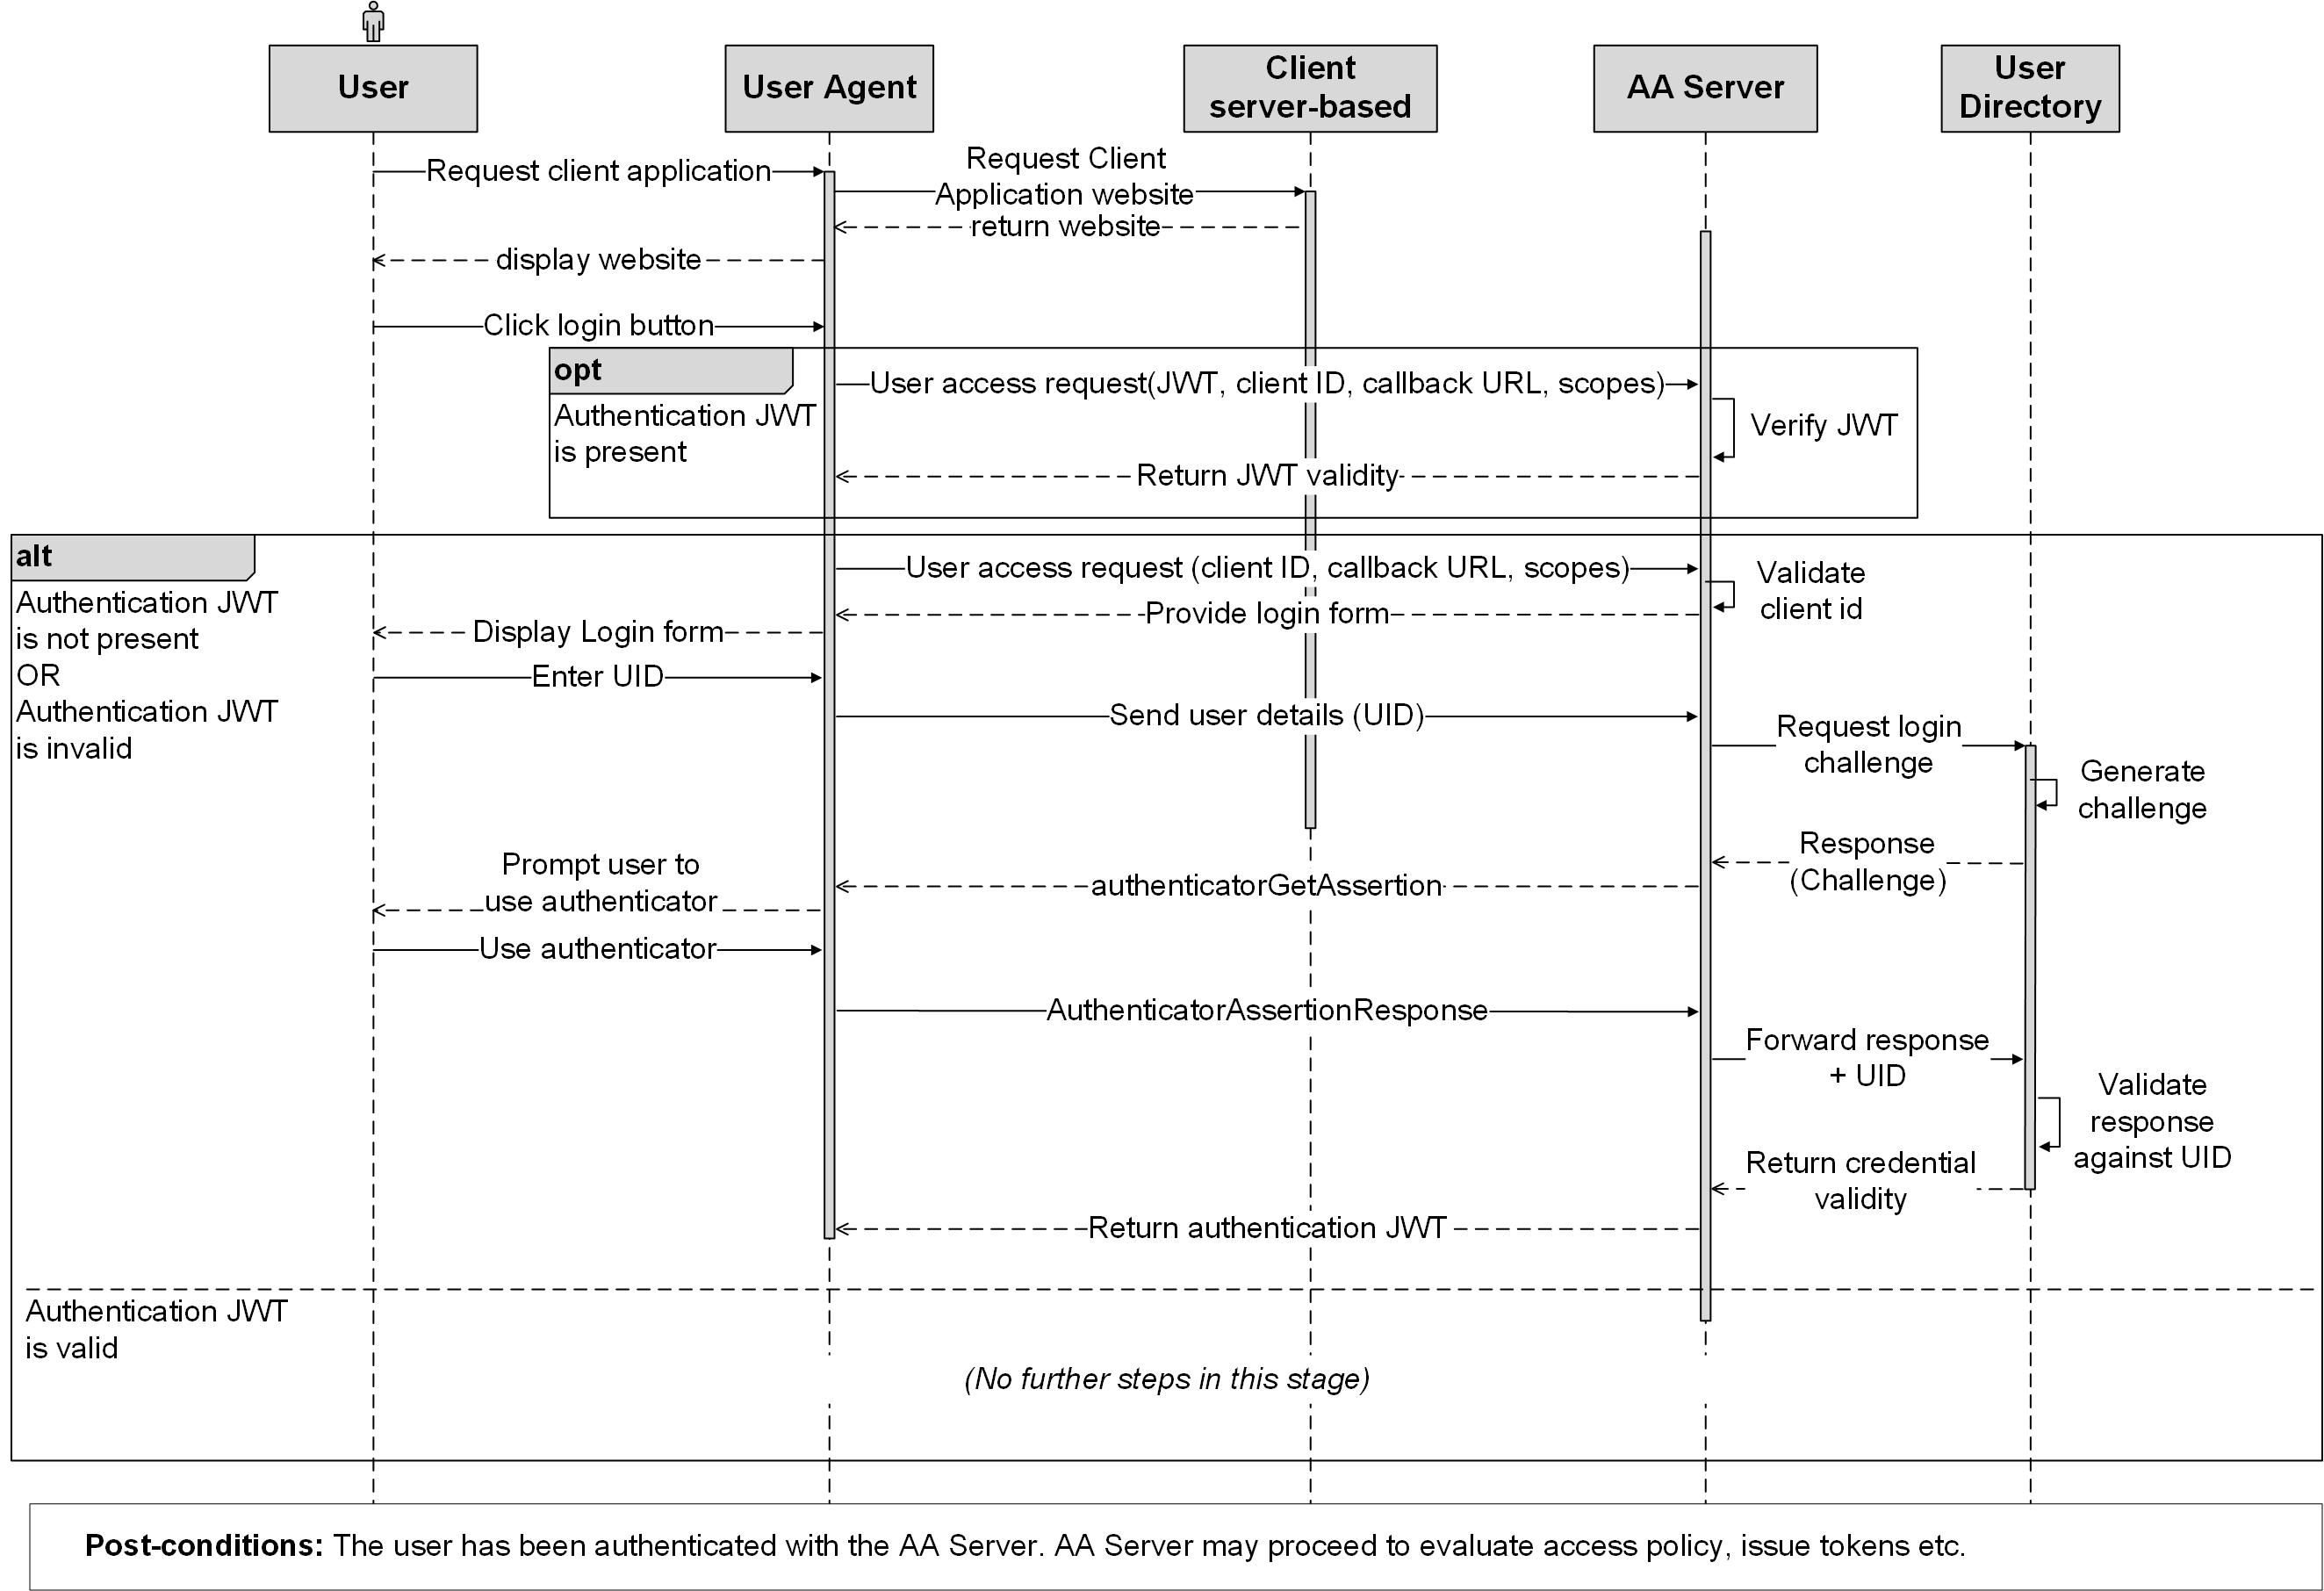
\includegraphics[width=\textwidth]{authentication-flow}
    \caption{Authentication flow during online access control with a server-based client, using a physical authenticator. If the authentication is not successful, the \acrshort{aaserver} informs the client and the user about the unsuccessful authentication and does not continue to the Access policy evaluation stage.}
    \label{fig:authentication-flow}
\end{sidewaysfigure}
\restoregeometry

\paragraph{Client authentication}
When a server-based client application requests access to resources that are not associated with an individual user, it must authenticate with the \acrshort{aaserver}, before the access is granted. OAuth documentation does not specify the form of this authentication~\cite{Hardt2012TheFramework}, but does permit the use of a client secret, that is only shared between the \acrshort{aaserver} and the client.

In the proposed system, client uses the client secret to authenticate with the server, before proceeding to the next stage.

\subsubsection{Access Policy Evaluation}
Once the authentication has been carried out, the \acrshort{aaserver} proceeds to the next stage -- Access Policy Evaluation. Involved in this stage are the \acrshort{aaserver}, the \acrshort{pdp} and, optionally the User Directory. The flow in this stage is the same when accessing an online application and the \acrshort{pacs}.

The flow begins by the \acrshort{aaserver} requesting access policy evaluation from the \acrshort{pdp} with an \textit{CheckAccessPolicy} message. Included in this request are the \acrshort{uid}, the \textit{client ID} (or \acrshort{pacs} identifier) and the context of the request. In the context, the environment and resource attributes are specified. If the \acrshort{pdp} can determine the policy based on these parameters, it issues the policy decision back to the \acrshort{aaserver}. If the \acrshort{pdp} cannot evaluate the policy directly, it can request further attributes about the user from the User Directory.

Figure~\ref{fig:policy-evaluation} shows these interactions in a sequence diagram. This stage is the same regardless of the Requester type. The Access Policy Evaluation stage concludes, when the \acrshort{pdp} informs the \acrshort{aaserver} about the policy decision. The \acrshort{aaserver} then proceeds to the Access Policy Enforcement stage.

\begin{figure}[H]
    \centering
    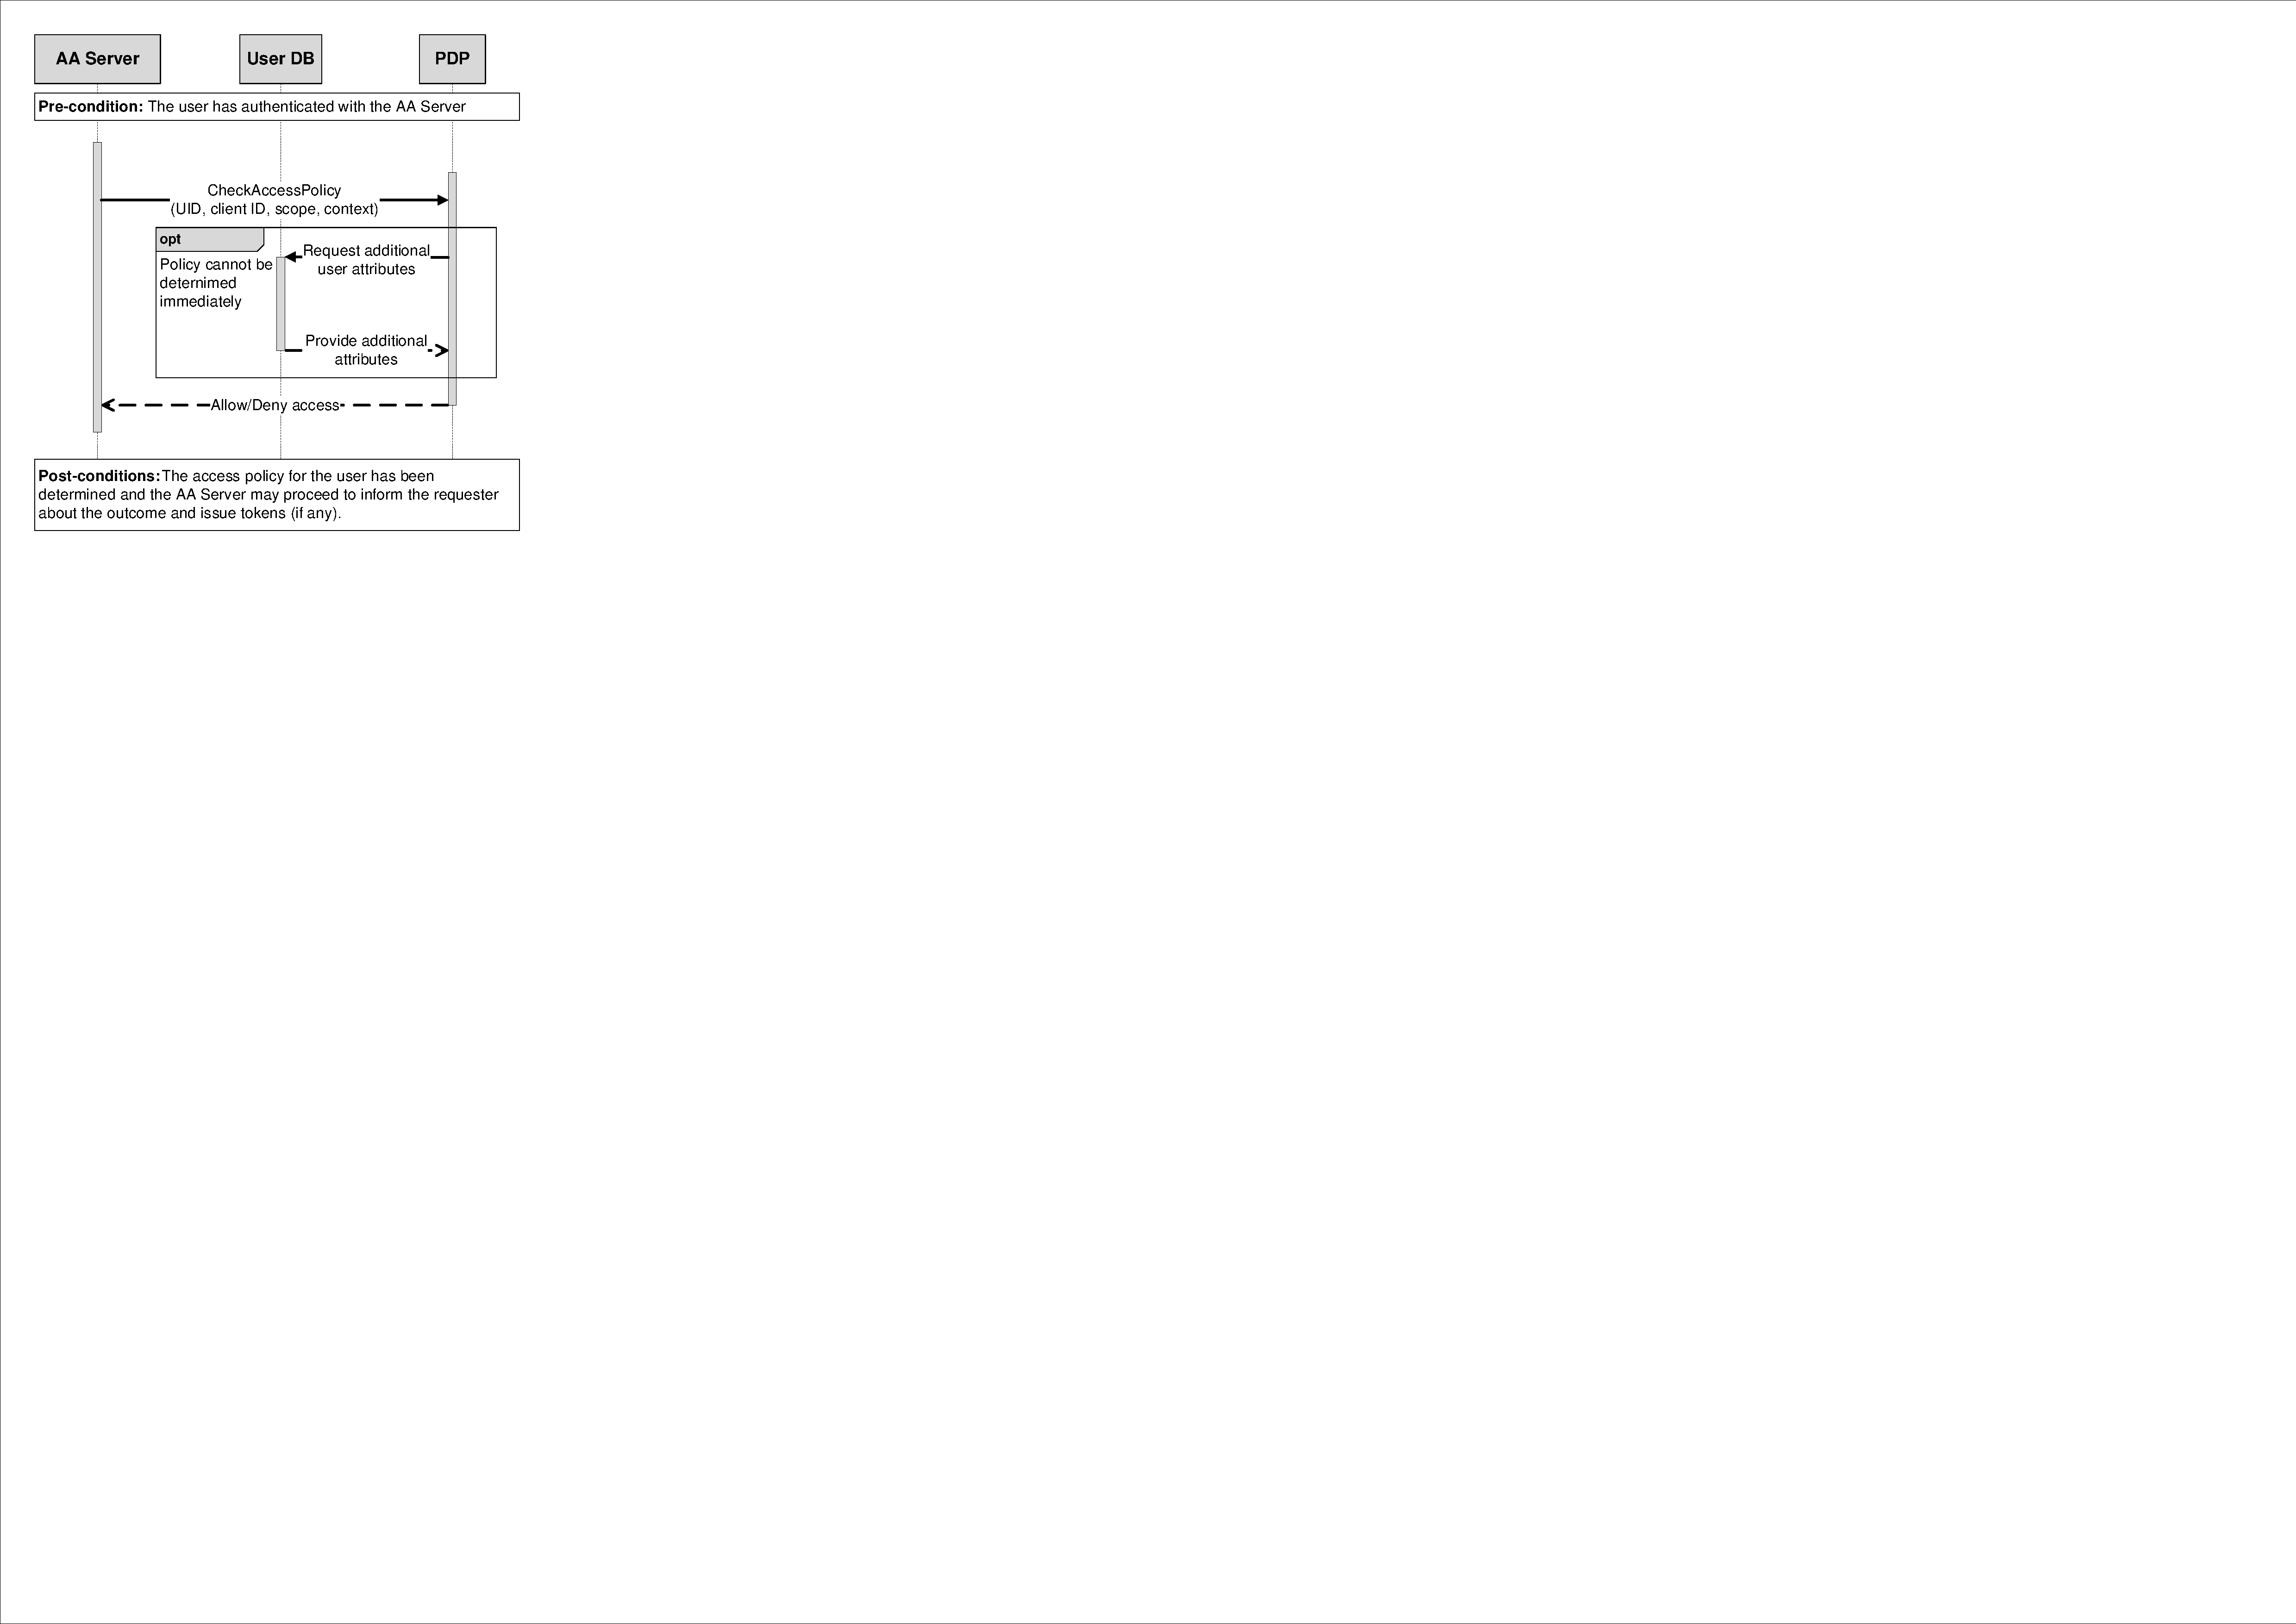
\includegraphics[width=.55\textwidth]{policy-evaluation2}
    \caption{Access Policy Evaluation stage. If a \acrshort{pacs} is the requester, then client ID is replaced with PACS ID (indicating which door is the user trying to open).}
    \label{fig:policy-evaluation}
\end{figure}

\subsubsection{Access Policy Enforcement}
The next stage in the access control flow is the Access Policy Enforcement. In this stage the policy decision is relayed to the Requester and tokens are issued (if any). The entities involved in this stage are the \acrshort{aaserver} and the Requester. The flow in this stage varies for different Requester types.

\paragraph{External client application}
If the policy allows access to the application, an ID token (as defined by~\cite{OpenID2014OpenID1}) is issued to sign the user in. If required by the client application, an access token, which permits access to user's protected resources, might also be issued. The client application indicates this in the \texttt{scopes} parameter of the \textit{UserAccessRequest} message.

To deliver the ID token (and Access token) to an external client application, Authorisation code grant is always used. If the client is a native or user-agent-based application, \acrshort{pkce} extension is used in addition, to lower the risk of the authorisation code spoofing by a malicious application residing at the user's device~\cite{Sakimura2015ProofClients}.

Once the ID token has been received and successfully verified by the client, the user is signed in using the information contained in the ID token, and may proceed to use the application. If necessary, the client application can use the access token to request additional information from the UserInfo endpoint. If the application requires manipulating with user's protected resources, it must include the access token in every request to the Resource endpoint.

If the policy denies user access to the application, the \acrshort{aaserver} informs the user agent and the client about this and does not issue any tokens. Figure~\ref{fig:accessing-resource-ext} illustrates this flow in a sequence diagram. The flow is different, if the client application is native or user-agent-based.

\paragraph{Internal client application and \acrshort{pacs}}
If the requester is an internal application or a \acrshort{pacs}, a token is not necessary to access protected resources. In this case, the \acrshort{aaserver} simply informs the requester about the policy decision and this decision is then enforced directly by the application/\acrshort{pacs}.

\bigskip\noindent
Due to many possible combinations of the authentication methods (smartphone, physical key), internal/external systems and client types (web-server based, user-agent based, native) we do not list all the possible flows in this section. Several additional diagrams are provided in Appendix~\ref{appendix:diagrams} for the following combinations:
\begin{itemize}[noitemsep, nolistsep]
    \item Opening door with physical key
    \item Opening door with a smartphone
    \item Accessing an external online system with a native client
    \item Accessing an external online system with a web-server based client
    \item Accessing an internal online system with a web-server based client
\end{itemize}

\bigskip\noindent
In this chapter, components of the proposed system and their functionality are presented. Selected use cases are described, which should be implemented in the prototype, demonstrating the functionality of the system. Flows during authentication, policy evaluation and policy enforcement document the exchange of information among the system components. These flows are used as an input to guide the implmentation, which is described in the following chapter.

\newgeometry{left=1.2cm,right=1.2cm,top=1cm,bottom=1cm,footskip=.4cm}
\begin{sidewaysfigure}[p]
    \centering
    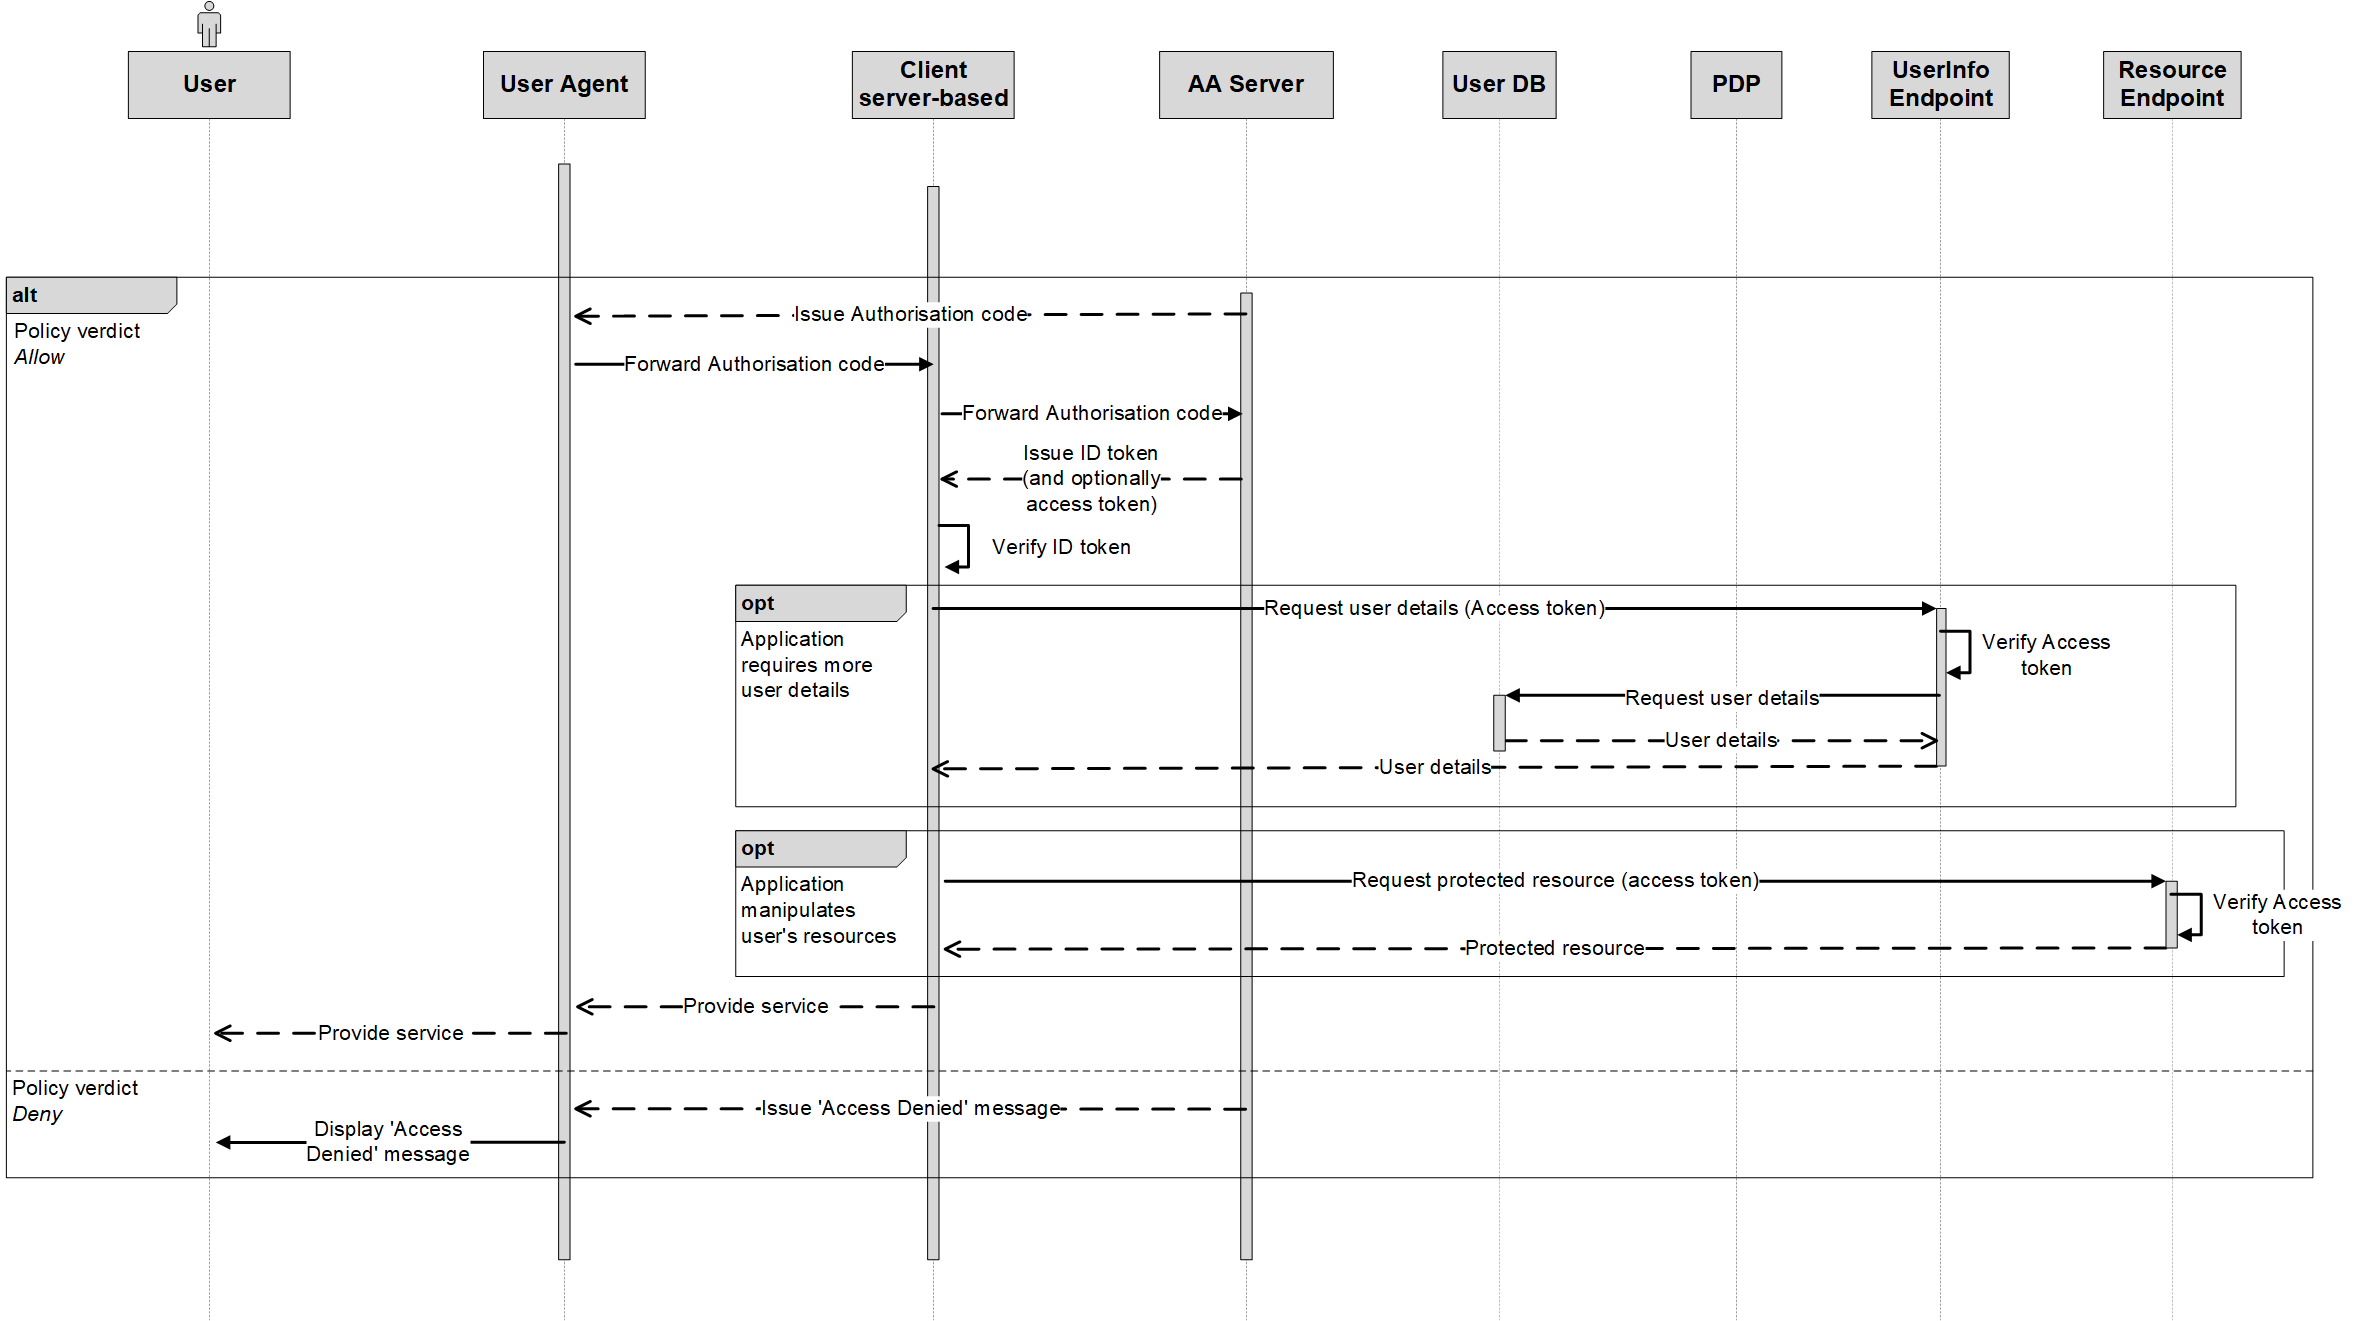
\includegraphics[width=\textwidth]{accessing-resource-ext}
    \caption{Sign-in and access token issuance process to external server-based client application.}
    \label{fig:accessing-resource-ext}
\end{sidewaysfigure}
\restoregeometry